\documentclass[11pt, a4paper]{article}
\usepackage[utf8]{inputenc}
\usepackage[left=2cm, right=2cm, top=2.5cm, bottom=2.0cm]{geometry}
\usepackage{amsmath, amssymb, amsthm}
\usepackage[english]{babel}
\usepackage{graphicx}
\usepackage[font={small,it}]{caption}
\graphicspath{ {figures/} }
\usepackage{url}
\usepackage[toc,page]{appendix}
\usepackage{float}
\usepackage[bottom]{footmisc}
\usepackage{titling}
\usepackage[numbered,autolinebreaks,useliterate]{mcode}
%\setlength{\droptitle}{-10em}  

\title{ \huge Artificial Neural Networks \\ 
  { \large Project 2: Hopfield networks: character recognition}}
\author{
        Lood, Cédric \\
        \small Master of Bioinformatics
}

\begin{document}
\maketitle

\section{Context}
The analysis presented in this report was done for the class of
Artificial Neural Networks at KU Leuven (Spring 2016). It consists in
a practical implementation of a hopfield networks with the goal to
investigate retrieval capabilities of such networks for alphabet. The
implementation was done in the MatLab environment (2015a) using the
neural networks toolbox. The scripts for each of the sections can be
found in the annex to this report.

\section{Hopfield network}

First we consider the creation of digital versions of characters. The
requirements were to build a sequence of characters (lowercase) using
our name + last name, followed by the uppercase alphabet. The
characters are represented by 7-by-5 matrices of 0s and 1s (0s being
interpreted as black, 1s as white). Figure \ref{fig:hopfield_chargen}
illustrates a sequence of such characters.

\begin{figure}[H]
  \centering
  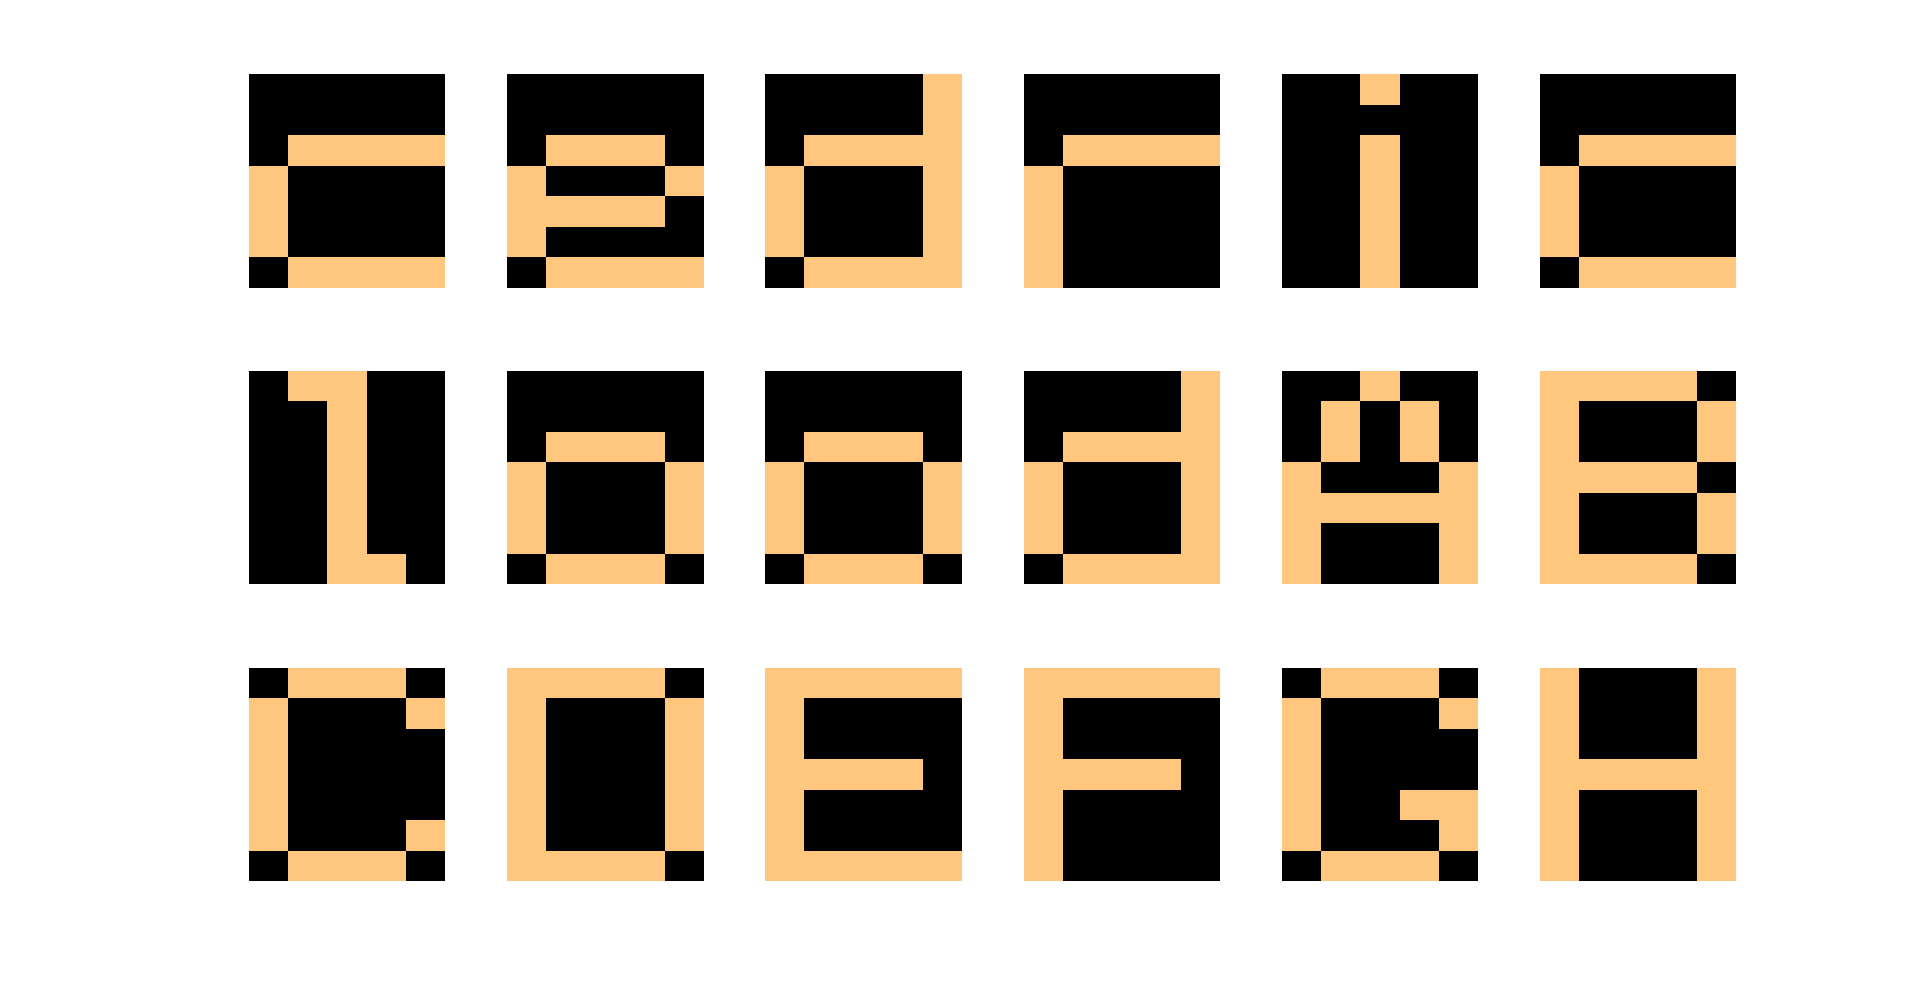
\includegraphics[scale=.30]{hopfield_chargen.png}
  \caption{Partial character sequence dataset}
  \label{fig:hopfield_chargen}
\end{figure}

An hopfield network was then created to store the first 5 letters of
the sequence as attractor points. One of the thing to keep in mind in
doing so is that the patterns that the hopfield net can store consists
of -1s and 1s, instead of 0s and 1s, so first a conversion needs to be
done. 

To test the retrieval of the points, some noise was added by flipping 3 random positions in the character, then presenting them to the network to see if they could be retrieved. This process is illustrated on figure \ref{fig:hopfield_chargen}

\begin{figure}[H]
  \centering
  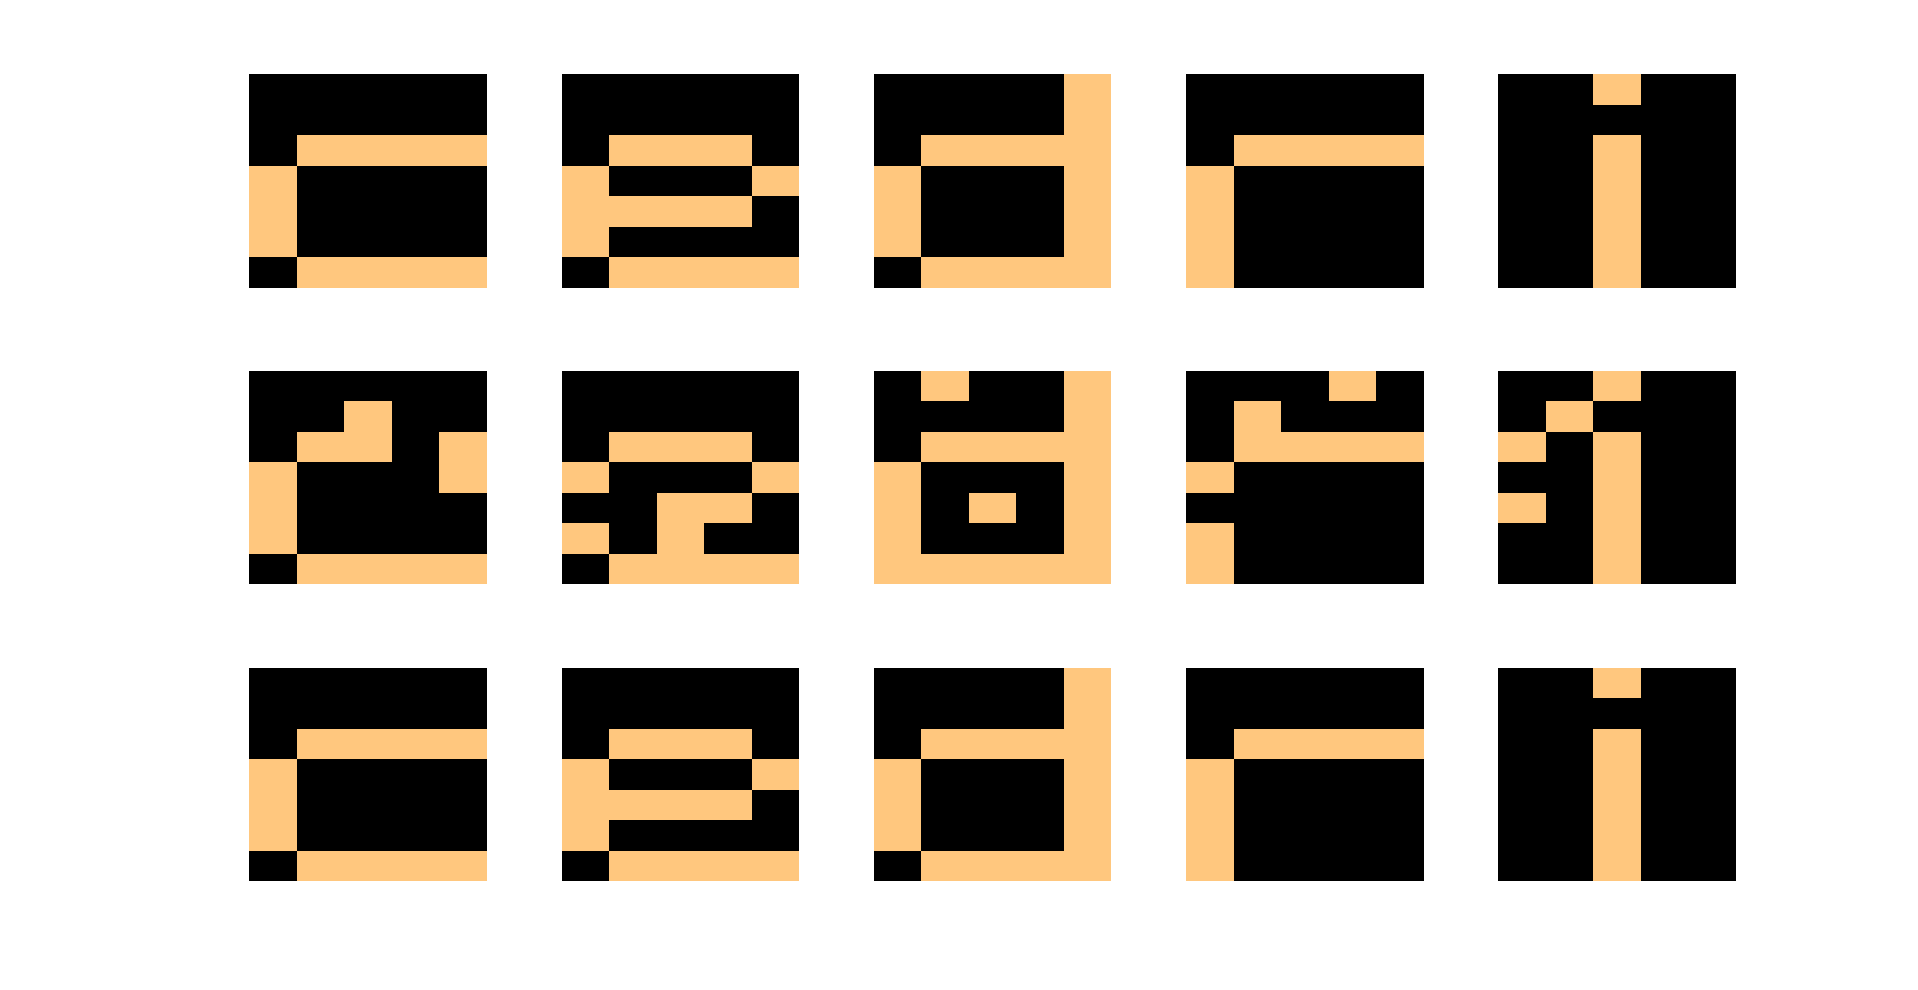
\includegraphics[scale=.30]{hopfield_denoising.png}
  \caption{Top: original letters, middle: added noise, bottom:
    retrieval from hopnet}
  \label{fig:hopfield_chargen}
\end{figure}

While the process did work perfectly, it is not immune to spurious
states. Those are states that are not explicitely put into the network
as attractors when it is build.

% \begin{figure}[H]
%   \centering
%   \includegraphics[scale=.43]{training_performance.pdf}
%   \caption{Training performance}
%   \label{fig:trainnl}
% \end{figure}

%{\footnotesize
%\bibliographystyle{ieeetr} 
%\bibliography{bib-db}}
\newpage
\begin{appendices}
\section{Hopnet}
\subsection{Part 1}
\begin{lstlisting}
clc, clear all, close all;
addpath 'export_fig'; % export pdf: https://github.com/altmany/export_fig
rng(7); % setting random seed

% generating data
%%%%%%%%%%%%%%%%%
characters = character_generator();
figure('Color', [1 1 1]);
for i = 1:18
    subplot(3,6,i);
    imagesc(reshape(characters(:,i),5,7)',[0,1]);
    axis off; colormap copper;
end

export_fig('hopfield_chargen.pdf');

% trick to rescal to -1 1 instead of 0 1 (requirement hopfield)
characters = 2*characters -1;

% Training network
%%%%%%%%%%%%%%%%%%
net = newhop(characters(:,1:5));

% plot original first 5 letters
figure('Color', [1 1 1]);
for i = 1:5
    subplot(3,5,i);
    imagesc(reshape(characters(:,i),5,7)',[0,1]);
    axis off; colormap copper;
end

% plot first 5 letters with noise
noisy_digits = zeros(35,5);
for i=1:5
    noisy_digits(:,i)=noise3(characters(:,i));
end
noisy_digits_plot = (noisy_digits+1)/2;
for i = 1:5
    subplot(3,5,i+5);
    imagesc(reshape(noisy_digits_plot(:,i),5,7)',[0,1]);
    axis off; colormap copper;
end

% reconstitute letters
for i = 1:5
    [Y Pf Af] = sim(net, {1 10}, [], {noisy_digits(:,i)});
    C = Y{1,10};
    recon_digits_plot = (C+1)/2;
    subplot(3,5,i+10);
    imagesc(reshape(recon_digits_plot(:,1),5,7)',[0,1]);
    axis off; colormap copper;
end
\end{lstlisting}
\subsection{Helper functions: character generator}
\begin{lstlisting}
function [characters] = character_generator()
c = [ 
    0 0 0 0 0 ...
    0 0 0 0 0 ...
    0 1 1 1 1 ...
    1 0 0 0 0 ...
    1 0 0 0 0 ...
    1 0 0 0 0 ...
    0 1 1 1 1 ]';
e = [
    0 0 0 0 0 ...
    0 0 0 0 0 ...
    0 1 1 1 0 ...
    1 0 0 0 1 ...
    1 1 1 1 0 ...
    1 0 0 0 0 ...
    0 1 1 1 1 ]';
d = [
    0 0 0 0 1 ...
    0 0 0 0 1 ...
    0 1 1 1 1 ...
    1 0 0 0 1 ...
    1 0 0 0 1 ...
    1 0 0 0 1 ...
    0 1 1 1 1 ]';
r = [ 
    0 0 0 0 0 ...
    0 0 0 0 0 ...
    0 1 1 1 1 ...
    1 0 0 0 0 ...
    1 0 0 0 0 ...
    1 0 0 0 0 ...
    1 0 0 0 0 ]';
i = [
    0 0 1 0 0 ...
    0 0 0 0 0 ...
    0 0 1 0 0 ...
    0 0 1 0 0 ...
    0 0 1 0 0 ...
    0 0 1 0 0 ...
    0 0 1 0 0 ]';
l = [
    0 1 1 0 0 ...
    0 0 1 0 0 ...
    0 0 1 0 0 ...
    0 0 1 0 0 ...
    0 0 1 0 0 ...
    0 0 1 0 0 ...
    0 0 1 1 0 ]';
o = [
    0 0 0 0 0 ...
    0 0 0 0 0 ...
    0 1 1 1 0 ...
    1 0 0 0 1 ...
    1 0 0 0 1 ...
    1 0 0 0 1 ...
    0 1 1 1 0 ]';   
characters = [c, e, d, r, i, c, l, o, o, d, prprob];
\end{lstlisting}
\subsection{Helper function: noise3}
\begin{lstlisting}
function [noisy_digit] = noise3(digit)
noisy_digit = digit;
[m, n] = size(digit);
noise = randperm(m);
noise = noise(1:3); % selects 3 positions to flip
for i=1:3
    noisy_digit(noise(i)) = -noisy_digit(noise(i));
end
\end{lstlisting}
\end{appendices}
\end{document}
